\section{3. Übungsblatt: $Relationen$, $vollständige\ Induktion$, $binomischer\ Satz$}

\subsection{Aufgabe 3.1}

\paragraph{(a)}
\begin{center}
\begin{tabular}{||c||c|c|c|c||c|c||}
\hline
\multicolumn{7}{||c||}{1 = ja, 0 = nein}\\
\hline
\hline
 & $reflexiv$ & $transitiv$ & $symmetrisch$ & $antisym.$ & Äquivalenzrelation & Ordnungsrelation \\
\hline
\hline
 $R_1$ & 1 & 0 & 1 & 0 & 0 & 0 \\
 $R_2$ & 1 & 0 & 0 & 0 & 0 & 0 \\
 $R_3$ & 1 & 1 & 1 & 0 & 1 & 0 \\
\hline
\end{tabular}
\end{center}

\paragraph{(b)}
$R$ umkehren und $x$, $y$ umkehren.

\newpage

\subsection{Aufgabe 3.2}
\begin{center}
\begin{tabular}{||c||c|c|c||c||}
\hline
\multicolumn{5}{||c||}{1 = ja, 0 = nein}\\
\hline
\hline
 & $reflexiv$ & $transitiv$ & $symmetrisch$ & Äquivalenzrelation \\
\hline
\hline
 (a) & 1 & 1 & 1 & 1 \\
 (b) & 1 & 0 & 1 & 0 \\
 (c) & 1 & 1 & 1 & 1 \\
\hline
\end{tabular}
\end{center}

$x-y\in\mathbb{Z}$ und $y-z\in\mathbb{Z}$, dnan $x-z=x-y+y-z\in\mathbb{Z}$\\

Äquivalenzklasse:\\

(a)\\
$xR_1y\Leftrightarrow x-\lfloor x\rfloor=y=\lfloor y\rfloor$\\
$\lfloor •\rfloor:\mathbb{R}\rightarrow\mathbb{Z}$, 
$x\mapsto\sup\{z\in\mathbb{Z}|z\leq x\}$\\
$R/R_1=\{[\alpha]|\alpha\in[0,1)\}$\\
$[\alpha]=\{\alpha+z|z\in\mathbb{Z}\}$\\

(b)\\
keine\\

(c)\\
Äquivalenzklasse sind immer TM von ganzen Mengen.\\
$[n]=\{n,-n\}\in\mathbb{Z}$, $\forall n\in\mathbb{N}$

\newpage

\subsection{Aufgabe 3.3}

\paragraph{(a)}
\begin{proof}
$ $\newline
Es sei:
\begin{equation*}
R\subset A\times A,\ S\subset A\times A
\end{equation*}
Aequivalenzrelationen\\

refl.:$\forall x\in A$, $(x,x)\in R$, $(x,x)\in S$, da:\\
$\Rightarrow$ $(x,x)\in R\cap S$ $\Rightarrow$ $R\cap S$ ist refl.\\

symm.:$\forall (x,y)\in R\cap S$,\\
$\Rightarrow$ $(x,y)\in R$, $(x,y)\\in S$ $\Rightarrow$(symm. von $S$ und $R$) $(y,x)\in R$, $(y,x)\in S$\\
$\Rightarrow$ $(y,x)\in R\cap S$\\

trans.:$\forall (x,y),(y,z)\in R\cap S$,\\
$\Rightarrow$ $(x,y),(y,z)\in R$ und $\in S$\\
$\Rightarrow$(transi. von $R$ und $S$) $(x,z)\in R\cap (x,z)\in S$\\
$\Rightarrow$ $(x,z)\in R\cap S$
\end{proof}

\paragraph{(b)}
\begin{center}
\begin{tabular}{|c|c|c|c|}
\hline
$R$ & a & b & c \\
\hline
a & x & x &   \\
b & x & x &   \\
c &   &   & x \\
\hline
\end{tabular}
\end{center}

\begin{center}
\begin{tabular}{|c|c|c|c|}
\hline
$S$ & a & b & c \\
\hline
a & x &   &   \\
b &   & x & x \\
c &   & x & x \\
\hline
\end{tabular}
\end{center}

\begin{center}
\begin{tabular}{|c|c|c|c|}
\hline
$R\cup S$ & a & b & c \\
\hline
a & x & x &   \\
b & x & x & x \\
c &   & x & x \\
\hline
\end{tabular}
\end{center}

$(a,b)\in R\cup S$, $(b,c)\in R\cup S$, $(a,c)\notin R\cup S$ contradiction.\\

\newpage

\subsection{Aufgabe 3.4}

\paragraph{(a)}
%$ $\newline

refl.: $\forall (\alpha, \beta)\in\mathbb{R}^2$, $\alpha\leq\alpha\wedge\beta\leq\beta$ gilt.\\

trans.: $\forall x,y,z\in\mathbb{R}^2$ wobei $x\leq y\wedge y\leq z$\\
$\overset{def}{\Rightarrow}$ $(x_1\leq y_1\wedge x_2\leq y_2)\cap(y_1\leq z_1\wedge y_2\leq z_2)$\\
$\Rightarrow$ $x\leq z$\\

anti.sym.: $\forall x,y\in\mathbb{R}^2$\\
s.d. $x\leq y\wedge y\leq x$\\
$\Leftrightarrow$ $(x_1\leq y_1\wedge x_2\leq y_2)\cap(y_1\leq x_1\wedge y_2\leq y_2)$\\
$\Rightarrow$ $x_1=y_1\wedge x_2=y_2$\\
$\Rightarrow$ $x=y$

\newpage

\subsection{Aufgabe 3.5}

\paragraph{(a)}
\begin{proof}
IA: $n=6$,
\begin{equation*}
2^6\cdot 6!=46080<6^6
\end{equation*}

IV: Sei für $n$ gilt $2^n\cdot n!<n^n$\\

IS: 
\begin{align*}
&2^{n+1}(n+1)!<(n+1)^{n+1}\\
=&2^n\cdot n!\cdot 2\cdot(n+1)
<2(n+1)\cdot n^n\\
\end{align*}
z.z $2<(1+\frac{1}{n})^n,\ \forall n>6$\\
(Binomische Satz.)
\end{proof}

\paragraph{(b)}
\begin{proof}
IA: $n=1$\\
\begin{equation*}
11^2+12=133
\end{equation*}

IV: $\exists k\in\mathbb{N}$, sodass $11^{n+1}+12^{2n-1}=133k$ für $n$ gilt.\\

IS:
\begin{align*}
\exists k\in\mathbb{N},\ sodass\\
11^{n+2}+12(2n+1)&=133\cdot k'\\
11\cdot 11^{n+1}+12^2\cdot 12^{2n-1}\\
11^{n+2}+12^{2n+1}&=11\cdot 11^{n+1}+12^2\cdot 12^{2n-1}\\
&=11\cdot 11^{n+1}+(133+11)\cdot 12^{2n-1}\\
&=11\cdot k\cdot 133+133\cdot 12^{2n-1}\\
&=11\cdot k\cdot 133+133\cdot 12^{2n-1}\\
&=133(11\cdot k+12^{2n-1})
\end{align*}
\end{proof}

\newpage

\subsection{Aufgabe 3.6(H)}

\paragraph{(a)}
\begin{proof}
$ $\newline

$reflexiv$\\
Sei $a\in M=\mathbb{Z}$, $a-a=0=5\cdot 0$\\
$\Rightarrow$ $(a,a)\in R_1$\\
$\Rightarrow$ $R_1$ $reflexiv$\\

$symmetrisch$\\
Sei $a,b\in M=\mathbb{Z}$ und $(a,b)\in R_1$\\
$\Rightarrow$ $\exists k\in\mathbb{Z}$, $a-b=5k$\\
mit $b-a=-(a-b)=-5k=5\cdot(-k)$, $\exists\tilde{k}=-k\in\mathbb{Z}$\\
$\Rightarrow$ $(b,a)\in R_1$\\
$\Rightarrow$ $R_1$ $symmetrisch$\\

$transitiv$\\
Sei $a,b,c\in M=\mathbb{Z}$, und $(a,b),(b,c)\in R_1$\\
$\Rightarrow$ $\exists k_1$, $a-b=5k_1$ und $\exists k_2$, $b-c=5k_2$\\
mit $a-c=a-b+b-c=5k_1+5k_2=5(k_1+k_2)$, $\exists\tilde{k}=(k_1+k_2)\in\mathbb{Z}$\\
$\Rightarrow$ $(a,c)\in R_1$\\
$\Rightarrow$ $R_1$ $transitiv$\\

$\Rightarrow$ $R_1$ ist Äquivalenzrelation auf $M$
\end{proof}

Äquivalenzklassen:

$[a]=\{x\in M\ |\ x=a-5k,\ k\in\mathbb{Z}\}$

$[b]=\{x\in M\ |\ x=b+5k,\ k\in\mathbb{Z}\}$

\newpage

\paragraph{(b)}
\begin{proof}
$ $\newline

$reflexiv$\\
Sei $a,b\in M$, $(a,b)\in M\times M$\\
mit $((a,b),(a,b)):a^2+b^2=a^2+b^2$\\
$\Rightarrow$ $((a,b),(a,b))\in R_2$\\
$\Rightarrow$ $R_2$ $reflexiv$\\

$symmetrisch$\\
Sei $a,b,c,d\in M$, $(a,b),(c,d)\in M\times M$, mit $((a,b),(c,d))\in R_2$\\
$\Rightarrow$ $a^2+b^2=c^2+d^2$\\
mit $((c,d),(a,b)):c^2+d^2=a^2+b^2\Leftrightarrow a^2+b^2=c^2+d^2$\\
$\Rightarrow ((c,d),(a,b))\in R_2$\\
$\Rightarrow$ $R_2$ $symmtrisch$\\

$transitiv$\\
Sei $a,b,c,d,e,f\in M$, $(a,b),(c,d),(e,f)\in M\times M$, mit $((a,b),(c,d)),((c,d),(e,f))\in R_2$\\
dann gilt
\begin{align*}
&a^2+b^2=c^2+d^2,\ c^2+d^2=e^2+f^2\\
\Rightarrow &a^2+b^2=e^2+f^2\\
\Rightarrow &((a,b),(e,f))\in R_2\\
\Rightarrow &R_2\ transitiv
\end{align*}

$\Rightarrow$ $R_2$ ist Äquivalenzrelation auf $M$
\end{proof}

Äquivalenzklassen:

Wir konstruieren eine Ebene $\mathbb{R}^2$, mit Koordinaten $x$ und $y$.

Dann $[a,b]=\{(x,y)\in M=\mathbb{R}\times\mathbb{R}\ |\ x^2+y^2=a^2+b^2,\ a,b,x,y\in\mathbb{R}\}$

d.h. nehmen wir beliebig $(a,b)$ aus $M$, dann haben wir in $\mathbb{R}^2$ einen Kreis mit Radius $a^2+b^2$.

Alle $(x,y)$, die aus Punkten von diesem Kreis besteht, erfüllt $(x,y)R_2(a,b)$.

Hier ein Beispiel:

\begin{figure}[h]
\centering
{
\fboxsep=0pt
\fboxrule=3pt
\fcolorbox{white}{white}{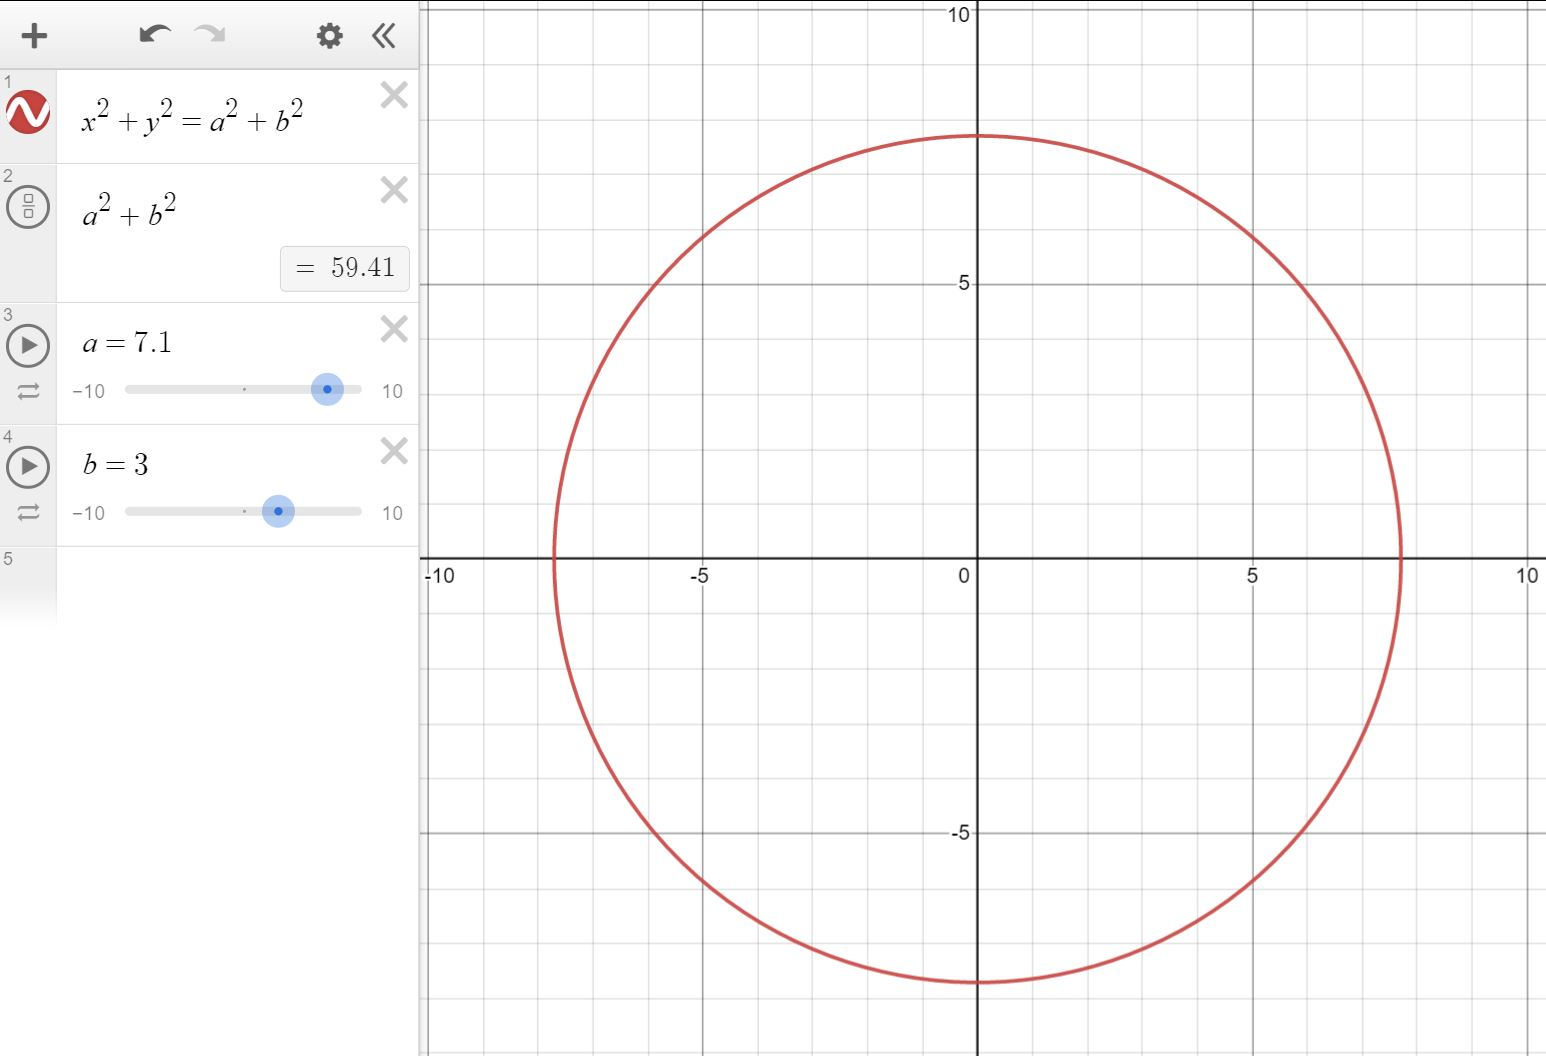
\includegraphics[width=12cm]{./pics/3.6b.jpg}}
}
\end{figure}

\newpage

\subsection{Aufgabe 3.7(H)}

\paragraph{(a)}
\begin{proof}
$ $\newline

IA: Sei $n=0$, es gilt:
\begin{equation*}
a_n=a_0=0+0+0=0\in\mathbb{N}
\end{equation*}

IV: $a_n=\frac{n}{6}+\frac{n^2}{2}+\frac{n^3}{3}$\\

IS: $\tilde{n}=n+1$\\
\begin{align*}
a_{\tilde{n}}=a_{n+1}=a_n
&=\frac{n+1}{6}+\frac{(n+1)^2}{2}+\frac{(n+1)^3}{3}\\
&=\frac{n+1}{6}+\frac{n^2+2n+1}{2}+\frac{n^3+3n^2+3n+1}{3}\\
&=\frac{n}{6}+\frac{n^2}{2}+\frac{n^3}{3}+\frac{1}{6}+\frac{2n+1}{2}+\frac{3n^2+3n+1}{3}\\
&\overset{\mathbf{IV}}{=}a_n+\frac{1}{6}+\frac{2n+1}{2}+\frac{3n^2+3n+1}{3}\\
&=a_n+\frac{6n^2+12n+6}{6}\\
&=a_n+n^2+2n+1\\
&=a_n+(n+1)^2\\
(n+1)^2\in\mathbb{N}&\Rightarrow a_n+(n+1)^2\in\mathbb{N}\\
&\Rightarrow a_{n+1}\in\mathbb{N}
\end{align*}
\end{proof}

\newpage

\paragraph{(b)}
\begin{proof}
$ $\newline

IA: Sei $n=0$, es gilt
\begin{equation*}
b_n=b_0=5^0-1=4\cdot k,\ k=0\in\mathbb{N}
\end{equation*}

IV: $b_n=5^n-1=4\cdot k,\ \exists k\in\mathbb{N}$\\

IS: $\tilde{n}=n+1$
\begin{align*}
b_{\tilde{n}}=b_{n+1}
&=5^{n+1}-1\\
&=5^n\cdot 5-1\\
&=5^n\cdot 5-1\cdot 5-4\\
&\overset{\mathbf{IV}}{=}5\cdot 4\cdot k-4\\
&=4\cdot(5\cdot k-1)\\
\exists\tilde{k}=5\cdot k-1\in\mathbb{N}&\Rightarrow b_{n+1}=4\cdot\tilde{k}\in\mathbb{N}
\end{align*}
\end{proof}

\paragraph{(c)}
\begin{proof}
$ $\newline

IA: Sei $n=0$, es gilt
\begin{equation*}
c_n=c_0=6^0-5\cdot 0+4=5=5\cdot k,\ k=1\in\mathbb{N}
\end{equation*}

IV: $c_n=6^n-5n+4=5\cdot k,\ \exists k\in\mathbb{N}$\\

IS: $\tilde{n}=n+1$
\begin{align*}
c_{\tilde{n}}=c_{n+1}
&=6^{n+1}-5(n+1)+4\\
&=6^n\cdot 6-5n-1\\
&=(6^n-5n+4+5n-4)\cdot 6-5n-1\\
&\overset{\mathbf{IV}}{=}(5\cdot k+5n-4)\cdot 6-5n-1\\
&=30k+30n-24-5n-1\\
&=5(6k+7n-5)\\
\exists\tilde{k}=6k+7n-5\in\mathbb{N}&\Rightarrow c_{n+1}=5\cdot\tilde{k}\in\mathbb{N}
\end{align*}
\end{proof}

\newpage

\subsection{Tutorium}

$M$, $N$ Mengen, $M\times N$\\
$R\subseteq M\times N$\\
Falls $\#M<\infty\wedge\#N<\infty$\\
z.B. $M=\{a,b\}$, $N=\{c,d\}$, dann $R=\{(a,c),(b,d)\}$ und $R^{-1}=\{(c,a),(d,b)\}$\\
